\documentclass[11pt, letterpaper, titlepage]{article}
\usepackage[utf8]{inputenc}
\usepackage[export]{adjustbox}
\usepackage{geometry}
 \geometry{
 a4paper,
 total={168mm,257mm},
 left=20mm,
 top=15mm,
 includefoot,includehead
 }


\usepackage[backend=biber, style=authoryear, giveninits=true, maxbibnames=25, uniquename=init, maxcitenames=2, hyperref=true, dashed=false]{biblatex}			% Benutze Biber/BibLaTeX zum Zitieren
\addbibresource{main.bib}					% Pfad zur BibTeX Datei aus Citavi
\renewcommand{\cite}{\parencite}
\usepackage{caption}
\usepackage{subcaption}
\usepackage{graphicx}
\usepackage{svg}
\usepackage{placeins}
\usepackage[hidelinks]{hyperref}
\usepackage{amsmath}
\usepackage[headsepline]{scrlayer-scrpage}
\usepackage{acronym}

\clearpairofpagestyles %Seitenzahl nicht in der Kopfzeile
\title{MeetEU Project - Team Heidelberg - Team 1 -- \\ Identification and Enhancement of novel Sars-CoV-2 NSP13 Helicase Inhibitors}
\author{Linda Blaier, Paul Brunner, Selina Ernst, Valerie Segatz, and Chlo\'{e} Weiler}
\date{February 2024}

%%%%%%%%%%%%%%%%%%%%%%% SELINA
\usepackage{tabularray}
\DeclareUnicodeCharacter{2009}{\,}

\begin{document}

\maketitle

\ihead{\headmark}
\automark{section}  %Kopfzeile gleich dem Sektiontitel
\cfoot{\pagemark}   %\ofood Seitenzahl rechts

\section{Abstract}
Even though the development of vaccines against Sars-CoV-2 was successful during the recent pandemic, the amount of FDA approved drugs for the therapy of Covid-19 is still limited to Paxlovid and Veklury, Olumiant and Actemra \cite{FDACOVID}. One possibility to accelerate the development of new therapies for Covid19 is to screen already approved drugs for effects against the viral reproduction. In this years MeetEU project, we investigated the NSP13 helicase of Sars-CoV-2 and tried to find compounds that could be repurposed for this therapy, as well as novel compounds that could lead to an effective treatment of Covid19. Using our \textit{in-silico} pipeline enables us to evaluate possible drug candidates, suggest novel structures based on already approved drugs and investigate their toxicity, while being cheaper and less labor intensive than projects limited to wet-lab work. 
\FloatBarrier

\newpage
%    Abkürzungsverzeichnis
{\setlength{\parskip}{0.2cm}
\section*{Abbreviations}
    \begin{acronym}[LC-MS/MS23]
        % A B C D E F G H I J K L M N O P Q R S T U V W X Y Z        
        % Abkürzungen
    \acro{COVID-19}{coronavirus disease 2019}
    \acro{FDA}{food and drug administration}
    \acro{MD}{molecular dynamics}
    \acro{MM-PBSA}{molecular mechanics energies combined with the Poisson-Boltzmann and surface area continuum solvation}
    \acro{NSP13}{non-structural protein 13}
    \acro{RMSD}{root mean square deviation}
    \acro{RMSF}{root mean square fluctuation}
    \acro{RTC}{replication transcription complex}
    \acro{SARS-CoV-2}{severe acute respiratory syndrome coronavirus type 2}
    \acro{SAscore}{synthetic accessibility score}
    \acro{ssRNA}{single-stranded RNA}
    \acro{Vina}{AutoDock Vina 1.1.2}
    \acro{ZBD}{zinc-binding domain}
       
        % Formelzeichen
        
        
        % als benutzt markierte Acronyme    
        
        
    \end{acronym}
}
\newpage
 
\section{Introduction}

\section{Material and Methods}

\subsection{Moecular Docking}
The molecular docking was done twice. 
% First as an initial screening of all 5092 prepared ligands (1472 from the ZINC database, 3620 from the ECBD database).
% ECBD pdbqt: 3813 (problematic: 193) = 3620 (size: 28) = 3592
% ZINC pdbqt: 1567 (problematic: 95) = 1472 (size: 44) = 1428
For the initial screening of the ligands \ac{Vina} was utilized \cite{Trott.2010}. As the receptor the monomer of 6ZSL was used which includes only chain A. Especially for \ac{Vina} the zinc ions were also removed and the resulting structure was converted into the pdbqt format through AutoDockTools 1.5.7 \cite{Goodsell2021}. The consensus pocket was introduced as the grid box with lengths of 30 \AA. The exhaustiveness was set to 30 and the maximum number of binding modes to 9. Taking advantage of multithreading, \ac{Vina} uses the 28 CPUs accessible on the multi-core server \cite{Che2023}. A filter was applied on the set of ligands assuring only 3D structures smaller than the specified grid box were screened against the receptor (1428 from the ZINC database and 3592 from the ECBD database). The filter was implemented in Python 3.11.6 and executed together with the \ac{Vina} command in Bash script. The resulting 9 different conformations for each ligand were ranked by their affinity scores and only the best value was considered in further steps. A number of ligands were later found to have multiple docking results due to an overlap between the two datasets and in accordance with previous steps only the best score was kept. The remaining 4862 ligands were ranked by their affinity score and the top one hundred were selected for next steps. \\
A second molecular docking was performed with those top scorers from the screening as well as ADP and ATP. The docking software Glide provided by Schrödinger Inc \cite{Friesner2004}. was accessed through Maestro 2022.3 \cite{Maestro2022}. The included tools Protein Preparation Wizard and LigPrep \cite{Madhavi2013} were utilized to prepare the monomer helicase and ligands for the docking process with the OPLS4 force field \cite{Lu2021}. The pH value was set to 7.0. The ligand preparation generates depending on the initial structure a varying amount of conformations. In the analysis of the results only the best performing conformation was included. The Receptor Grid Generation panel was used to generate the receptor grid with the same binding pocket as in \ac{Vina}. The docking with Glide was performed at standard precision (SP) mode and with flexibility of the ligands enabled \cite{Halgren.2004}. The criteria for the selection of the best performing ligands was chosen to be the docking score. The interactions between the top scoring ligands and the receptor were noted down. 


\section{Results}

\subsection{Screening of ligands with AutoDock Vina}
A library of 5020 ligands was screened against the consensus binding pocket of the NSP13 helicase. The best conformation with the lowest binding affinity was determined for each one of these ligands. 157 of them were included two or three times. The respective difference of affinity between the multiple forms of each ligand never exceeded 1.6. In 24.2 \% of these cases the affinity score remained the same. Whenever the difference is not equal to zero the corresponding rank of the affinities changed with a maximum margin of 2966. In the case of multiple runs for each ligand the best scoring docking result was kept. The remaining 4862 had affinity values ranging from -10.3 to -2.4. The ranking of the ligands was determined by their affinity which lead to the selection of the top one hundred ligands. Their values ranged from -10.3 to -8.8. Containing 2.1 \% of all ligands these top scorers are only the preselection for the subsequent docking process. 

<<<<<<< Updated upstream
\subsection{Molecular Docking of top scorers with Glide}
=======
\subsection{Molecular Docking Top scorers with Glide}
>>>>>>> Stashed changes
The 100 top scorers from the screening were subjected to another molecular docking to the NSP13 helicase. The resulting docking scores from Glide were utilised to establish another ranking. The comparison of the results from Vina and Glide showed that there was no correlation between these ranks (\autoref{fig:comp_glide_vina}). The Pearson correlation coefficient r of the scores is 0.13 with a p-value of 0.19 which is similar to the r value of the ranks at 0.12 with a p-value of 0.22. The Kendall correlation coefficient computed by comparing the ranks only is 0.07 with a p-value of 0.25. In all three cases it is not possible to reject the null hypothesis of no correlation. Even so, there are 3 from the top 5 Vina scorers (rank 1, 2 and 4) that are also part of the top 10 (rank 9, 10 and 8) according to Glide. Moving forward docking scores from Glide are the preferred selection criteria since Glide provided flexibility of ligands and the retainment of the protein zinc ions. \\

% for appendix
\begin{figure}[htp]
	\centering
	\captionsetup[subfigure]{skip=-20pt,position=top,labelfont=bf,labelformat=parens,singlelinecheck=false}
	\subcaptionbox{%
		\label{subfig:comp_ranks}}{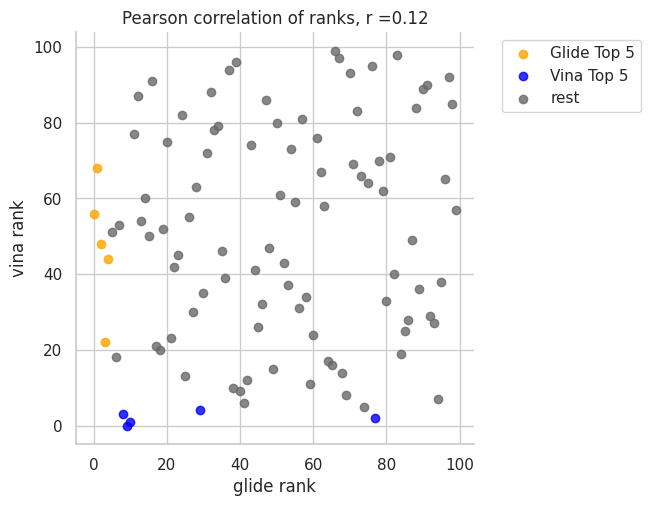
\includegraphics[scale=0.5]{Comparison_of_ranks.png}}
	\subcaptionbox{%
		\label{subfig:comp_scores}}{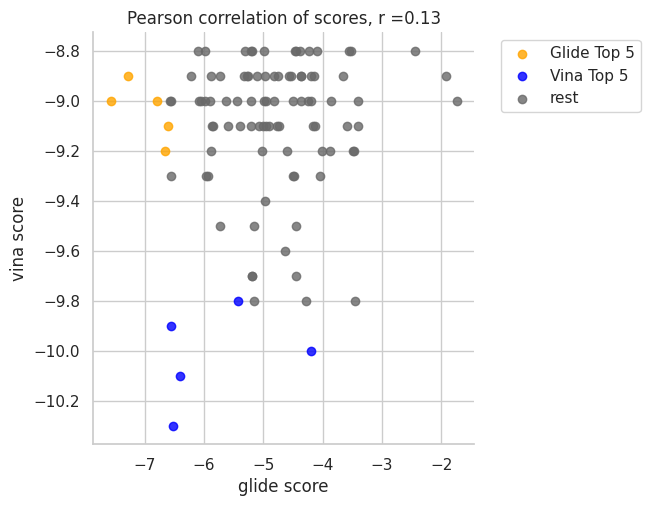
\includegraphics[scale=0.5]{Comparison_of_scores.png}}
	\caption{Comparison of Vina and Glide docking results. 100 ligands were compared in  \subref{subfig:comp_ranks}) ranks and \subref{subfig:comp_scores}) docking scores. Dots in blue represent the top 5 ligands from Vina and in orange the top 5 from Glide. All the other ligands are marked green.}\label{fig:comp_glide_vina}
\end{figure}

<<<<<<< Updated upstream
The potential lead compounds defined in this way are as follows: Angiotensin 1-7 (ECBD ID: EOS100380, ZINC ID: ZINC000096077632), ZINC000008101127 (ECBD ID: not existent) and VX-11 (ECBD ID: EOS100897, ZINC-ID: ZINC000035880991). Each one of these ligands has a better docking score and therefore higher affinity to the receptor than ADP (\autoref{tab:top_docking_scores}). However ATP still binds better than any one them.
=======
The potential lead compounds defined in this way are as follows: ZINC000096077632 (ECBD ID: EOS100380, popular name: Angiotensin 1-7), ZINC000008101127 and ZINC000035880991 (ECBD ID: EOS100897, popular name: VX-11). Each one of these ligands has a better docking score and therefore higher affinity to the receptor than ADP (\autoref{tab:top_docking_scores}). However ATP still binds better than any one them.
Another output are the iintermolecular interactions between the small molecules and the receptor binding pocket. Interesting to note is that especially ATP, ADP and the highest top scorer ZINC000096077632 have many common 
bonds with the amino acids like LYS 288, LYS 320 and ARG 443 (\autoref{tab:ligand_interactions}). In most cases these bonds are either hydrogen bonds or salt bridges with some exceptions like an aromatic hydrogen bonds, halogen bonds or pi-cation. One amino acid in particular stands out which is LYS 288 that also interacts with the other top 3 scorers ZINC000008101127 and ZINC000035880991. 
When comparing the overall positions of ZINC000096077632 (\autoref{fig:docking_EOS100380}) and ADP (\autoref{fig:docking_ADP}) within the binding pocket the similarities are even more apparent. 


%
%\subsection{Comparison of AutoDock Vina results}
%%This part only makes sense if they actually used the same pocket? Don't think they used the same 6zsl structure ...
%The Team Sorbonne5 also used AutoDock Vina for the docking of ligands from the pilot library of the ECBD database. Most of these ligands were also included in the former mentioned analysis. With the exception of two it is possible to map the top 10 ligands from Sorbonne to results of the analysis. Only one of their top scorers is included in the 100 preselected ligands. Their first ranked ligand with the affinity score -11.1 has a corresponding rank of 63. The remaining 7 were mapped to lower ranks starting with 123 and ending with up to 2626.
%
%\subsection{Validation of binding-site for the Top10 scorer of Glide}
%As shown in \autoref{pymol_Top3}, Diffdock did not validate our binding site for our Top 1 and Top 2 glide results. None of the predicted conformations Diffdock was most confident in were found within our designated binding site. For our Top 3 Glide result on the other hand, at least two of the 10\% ranked best by Diffdock seem to have interaction with our binding site and are defined as being within our binding pocket. Furthermore, Diffdocks confidence into conformations of our Glide Top 3 ligand seems to correlate with their position within our binding pocket (Supplementary Material \autoref{Diffdock_plot}). This findings supports the assumption that the preferred binding site for this ligand is within our binding pocket. Among our Top 10 Glide ligands, better results according to Diffdock were only achieved for our Top 5 Glide ligand.
%\begin{figure}[htp]
%	\centering
%	\captionsetup[subfigure]{skip=-15pt,position=top,labelfont=bf,labelformat=parens,singlelinecheck=false}
%	\subcaptionbox{%
%		\label{subfig:top1_glide_diffdock}}{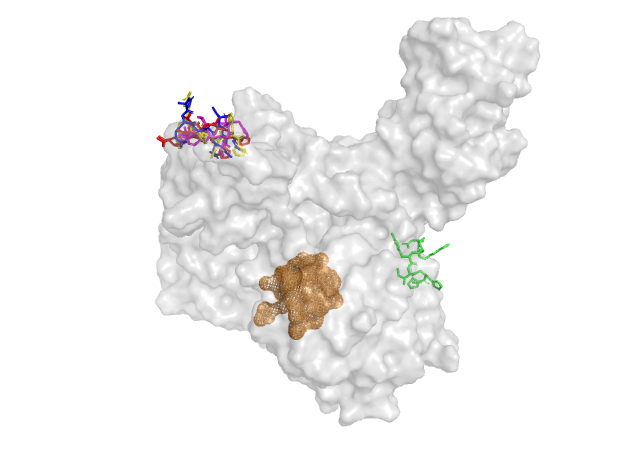
\includegraphics[scale=0.24]{Top1_Glide_Rank5}}
%	\subcaptionbox{%
%		\label{subfig:top2_glide_diffdock}}{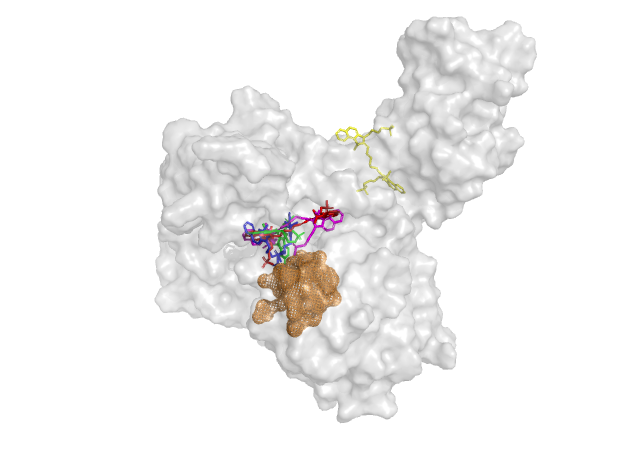
\includegraphics[scale=0.24]{Top2_Glide_Rank5}}
%  	\subcaptionbox{%
%		\label{subfig:top3_glide_diffdock}}{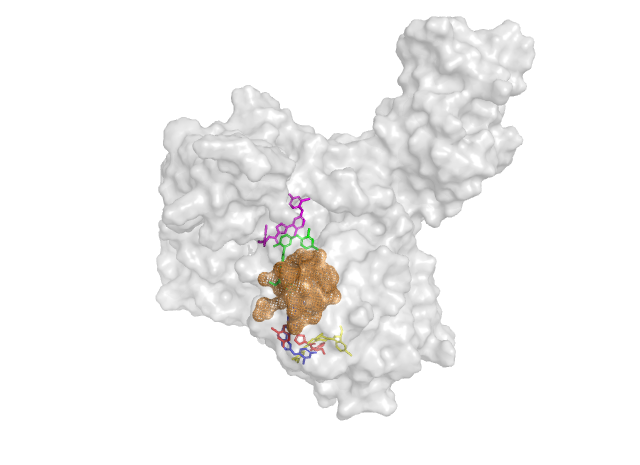
\includegraphics[scale=0.24]{Top3_Glide_Rank5}}
%	\caption{Diffdock results for our Top 3 Glide ligands. Shown are always the 5 ligand conformations Diffdock was most confident in. (a) Glide Top-1 (b) Glide Top-2 and (c) Glide Top-3.}\label{pymol_Top3}
%\end{figure}
%
%\subsection{Top 100 Compounds Exhibit Low Toxicity and High Synthetic Accessibility}
%After identifying the top 100 best-binding ligands through AutoDock Vina, our subsequent analysis focused on evaluating their practical applicability as potential drugs by considering their predicted toxicity and synthetic accessibility. The resulting SAscore and Tox-Score for each compound were visualised in a scatter plot as seen in {Figure \ref{eToxPred}}. 
%
%\begin{figure}[h]
%    \begin{center}
%      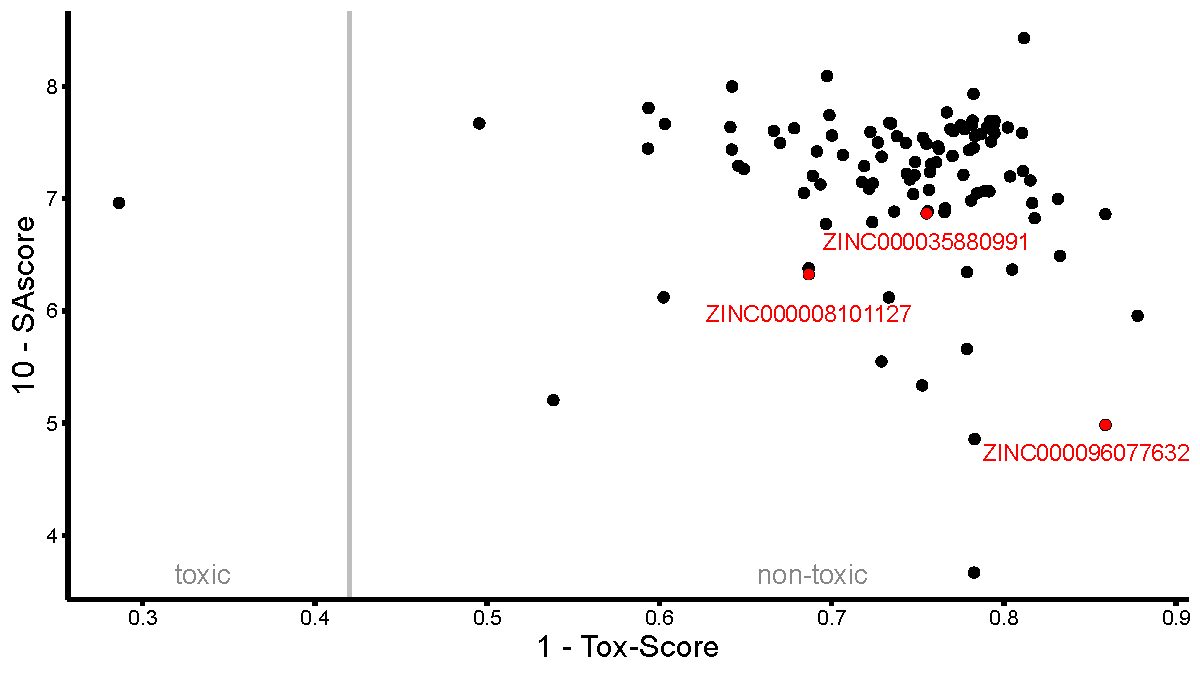
\includegraphics[width=0.78\textwidth]{etoxpred_result.pdf}
%    \end{center}
%    \caption{\textbf{Scatter plot of predicted toxicity and synthetic accessibility of the 100 best-binding compounds.} The predicted \ac{SAscore} was plotted against the Tox-Score for the top 100 best scorers from AutoDock Vina. The top 3 scorers from Glide are highlighted in red. The vertical gray line represents the threshold for the toxicity, with the compounds to the right of this line being considered non-toxic.}\label{eToxPred}
%  \end{figure}
%
%\noindent Of those 100 compounds, 99 presented with a Tox-score below the threshold of toxicity, indicating a low probability of being toxic to humans. The overall median Tox-Score is 0.24, with a mean of 0.26 across all compounds. Across all compounds the median SAscore of 2.69 and a mean of 2.87 which suggests that they are genereally easy to synthesise. The top scorer from Glide, ZINC000096077632, was predicted to have a Tox-Score of 0.14 and an SAscore of 5.02.
%
%
%\subsection{Molecular Dynamics Simulation Validates Binding of Top Scorer}
%The \ac{MD} simulation is integral to validate the results of our pipeline. After the production run was finished, the resulting trajectory file was centred on the protein and modified to remove any ghosting and splitting of the protein at the borders of the simulation box. The last frame of the simulation was extracted and visualized using \textit{pyMOL} \cite{PyMOL}, which can be seen in Figure \ref{MD.Annotated}.
%\begin{figure}[h]
%  \begin{center}
%    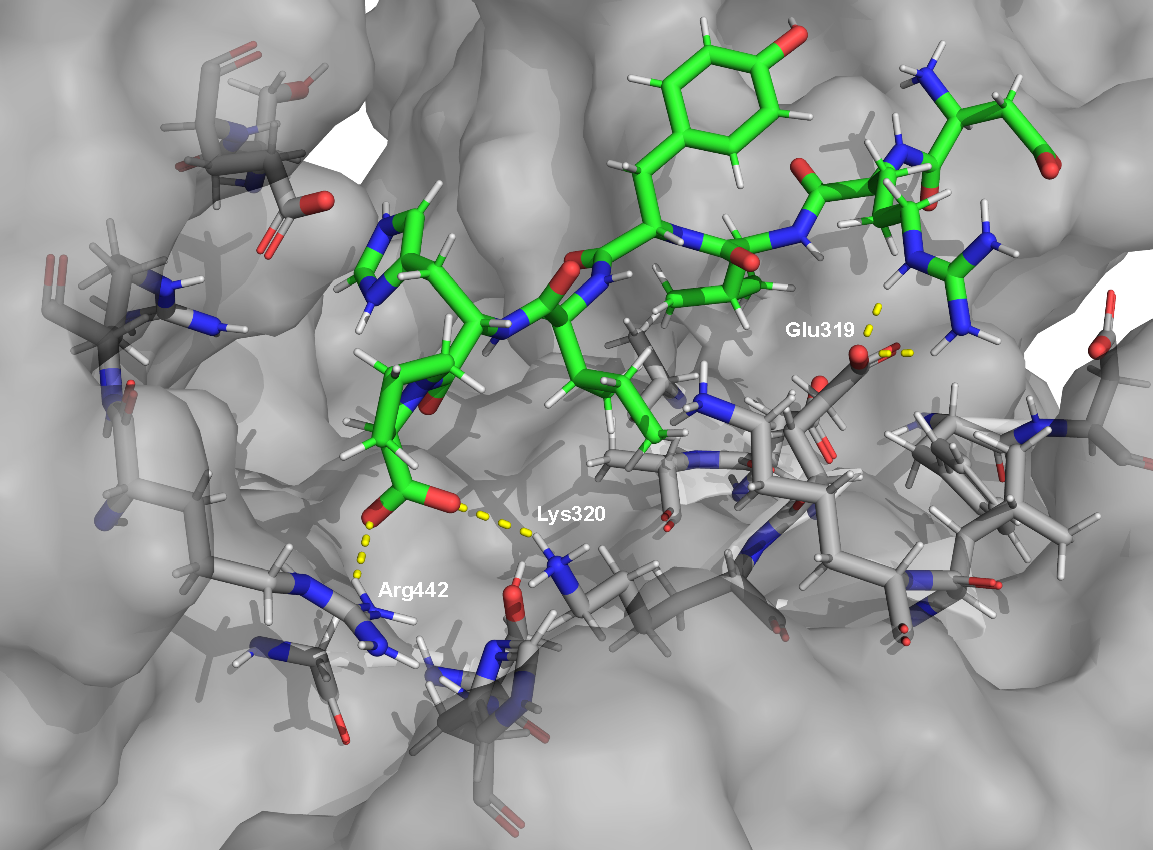
\includegraphics[width=0.8\textwidth]{last_frame_render_annotated.pdf}
%  \end{center}
%  \caption{\textbf{Visualisation of EOS100380 inside the binding pocket at the end of 100 ns simulation.} The polar interactions are marked with yellow dotted lines. The amino acids involved in these interactions are labelled.}\label{MD.Annotated}
%\end{figure}
%The figure clearly demonstrated, that the top scoring compound of our Glide screening stayed inside of the binding pocket until the end of the simulation. This was also confirmed by manual inspection of the frames generated in the simulation, which were combined to a video file using \textit{VMD}. Furthermore, the polar interactions between the ligand and residues in its proximity are shown. It seems, that EOS100380 is bound to the protein by interactions with Glu319, Lys320 and Arg442 of the NSP13 helicase. These interactions could also be validated using \textit{LigPlot+} \cite{LigPlot}.\\
%To investigate the dynamics of these interactions between ligand and protein, the \ac{RMSD} and \ac{RMSF} were calculated, which can be observed in Figure~\ref{rms}. 
%\begin{figure}[h]
%  \begin{center}
%    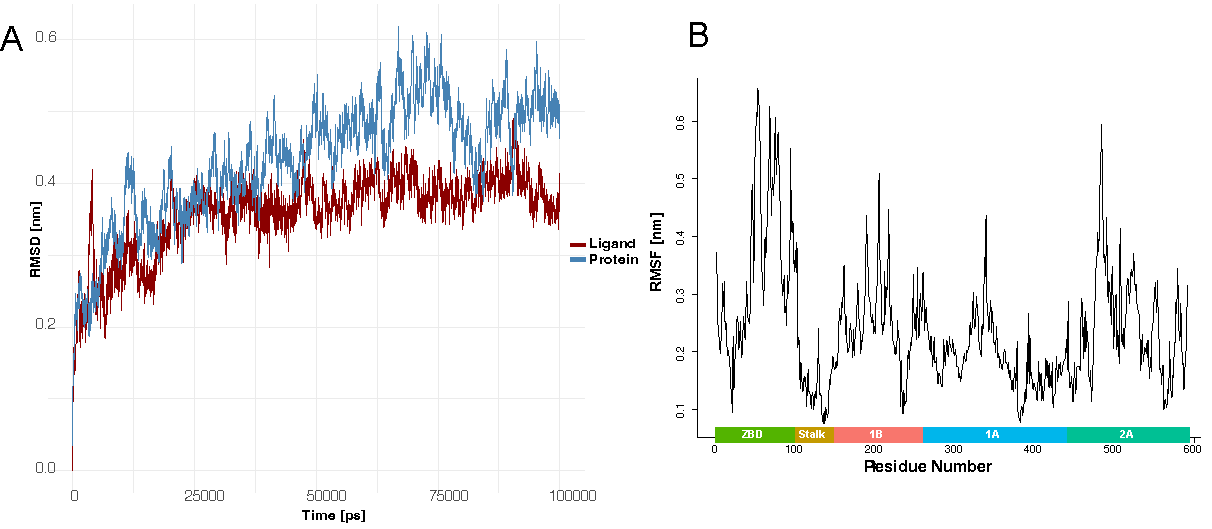
\includegraphics[width=1.0\textwidth]{RMSD_RMSF_combined.pdf}
%  \end{center}
%  \caption{\textbf{RMSD of the protein backbone and ligand (A) and RMSF of the protein backbone per residue during the simulation (B).} The RMSD was plotted over time for the whole 100 ns simulation. The respective RMSDs are shown in red (ligand) and blue (protein) The RMSF is shown per residue in the residue. The colour bar annotates the protein domain the respective residue belongs to, according to \textcite{Domains}. ZBD = Zinc Binding Domain}
%  \label{rms}
%\end{figure}
%The \ac{RMSD} observed over the course of the simulation (Figure~\ref{rms}A) rises at first, but reaches a plateau in both the ligand and the protein. The RMSD seems to settle faster in the ligand, which exhibits less movement in general. Investigation into the RMSF per residue (Figure~\ref{rms}B) suggests, that some residues move significantly more than others. The highly mobile residues seem to be located in the zinc binding domain and domains 1B and 2A. The latter two play a role in the binding of the ligand. Thus movement in these parts of the protein was to be expected. All in all, the protein and ligand seems to undergo conformational changes, however the system does not show major signs of instability. The ligand seems to settle in a somewhat stable conformation after roughly 50ns. More information on the movement of the protein can be seen when investigating the radius of gyration (Supplementary Figure \ref{gyr}). The estimation of the interaction energy by MMPBSA returned a $\Delta G_{solv} = -9.98 \frac{\textrm{kcal}}{\textrm{mol}}$. The RMSD and RMSF of the simulation using ANP as the ligand can be seen in Supplementary Figure \ref{anp}. The system shows a generally lower RMSD and an earlier plateau compared to the first simulation. For the RMSF a similar trend can be observed, especially looking at the ZBD. 
%%renew after cs2

\FloatBarrier

\section{Discussion and Outlook}
The Vina search algorithm produces randomly altered conformations of the ligand molecule which impacts the affinity values and the rank. Other factors that have impact on the ranking are the rigidness of molecules and the missing zinc ions of the protein. For these reasons Glide results were chosen as the main contributor for selecting the top scorers. Both Vina and Glide are computational methods to predict optimal docking conformations but are limited by their assumptions of physical properties of the molecules. 

Only one of the top scorers from the Sorbonne 5 team, which used the same pilot library from ECBD, was included in the top 100 established through Vina and placed 73rd place in the Glide ranking. That can be expected since a different binding pocket was used.

paper compares glide and vina
Glide: flexible ligands, zinc ions, generally better because same molecule produces same score, 


The Tox-Score predictor of \textit{e}ToxPred was trained using \ac{FDA}-approved dataset as non-toxic incidences. Consequently, the low mean Tox-Score of the tested compounds aligns with our expectation, considering that the compounds from the ZINC database are derived from an \ac{FDA}-approved dataset. The single toxic incidence we detected was from the ECBD database which was comprised of \ac{FDA}-approved and non-\ac{FDA}-approved molecules.
As highlighted by \citeauthor{pu2019toxpred}, natural compounds typically exhibit higher \ac{SAscore} values compared to synthetic compounds due to their inherent complexity \cite{pu2019toxpred}. The relatively high \ac{SAscore} of ZINC000096077632 can be explained by the fact that ZINC000096077632 corresponds to angiotensin-(1-7) which is a naturally occuring compound with a crucial role in the \ac{RAS} \cite{santosangiotensin}. The analysis of natural compound datasets by \citeauthor{pu2019toxpred} revealed a bimodal distribution in the \ac{SAscore}, with peaks around 3 and 5. Furthermore the very low Tox-Score of the top scorer can also be explained by the fact that it is a naturally occuring molecule in the human body. \\

\noindent The investigation into the \acf{MD} simulation further validated the viability of our pipeline. The RMSD of the backbone protein atoms (see Figure~\ref{rms}A) was slightly higher than anticipated, as it seemed to generally be smaller in the tutorials provided by \citeauthor{Lemkul2018}. However, the system stabilised over the duration of the simulation. Looking at the RMSF per residue (see Figure~\ref{rms}B) it is apparent, that certain domains of the protein lead to this increase in the RMSD. Especially the zinc binding domain shows a lot of movement. When discussing the general movement of domains in such simulations one should keep in mind, that the NSP13 A-chain is part of a much bigger replication complex \cite{NSP13_basics} in an \textit{in-vitro} setting. The conformational changes seen in this analysis would be severely hindered by other components in the complex. The domains 1B and 2A were suspected to be involved in a lot of conformational changes, as they make up a large part of the interaction surface between the protein and the ligand. The RMSD is calculated versus the output of Glide as a reference structure. It is completely possible that the system created by Glide is not completely relaxed. Thus conformational changes are to be expected when protein and ligand can suddenly move freely. Investigating the RMSD of the ligand shows, that it too settles in a stable conformation during the simulation time span. Some of the RMSD can be attributed to functional groups far away from the binding site rotating along their sigma bounds, which was observed during manual inspection of the simulation. All in all, the analysis offers confidence, that EOS100380 binds to the NSP13 helicase and stays bound through an extended period of time. This fits the work of \textcite{angio}, who propose Angiotensin 1-7 as a new therapy to support the recovery from Covid-19. Next to its role in the Renin-Angiotensin-Aldosteron System, it seemingly could also lower the viral damage to the body by inhibiting NSP13.



\section{Limitations of the project}
Regarding the \acf{MD} simulation, the project was held back by the tight time schedule of the Meet-EU seminar. Running simulations for other top scoring ligands would have helped immensely in validating out pipeline further and compare the results of the top scorer. Running multiple runs of the same simulation would have also further deepened our confidence in the results, as MD simulations in and of them selves are a very stochastic process and should always be estimated using replicas. Following the work of \textcite{REDS}, implementing replica exchange with dynamical scaling would have elevated the validation step of this project. Access to more GPUs would have also made multiple simulations at once possible.
For the analysis of the protein-ligand complex using \textit{gmxMMPBSA} the same calculation should have been conducted on the MD run using ANP as the ligand. However, due to technical difficulties the calculation could not be performed in time. Thus the given $\Delta G_{solv}$ of our ligand is a little bit difficult to interpret without a comparison value.
Furthermore, the original plan to implement \textit{AutoGrow4} \cite{packageAutogrow4} in order to improve our lead drugs and generate novel compounds was hindered by technical problems, which could not be fixed with the limited time at our disposal. We believe, that the increase in diversity amongst the drug candidates would lead to a better final drug candidate. With the help of \textit{eToxPred}, as shown in this report, the new compounds could have been evaluated for their toxicity and a well binding, not too cytotoxic lead could have been presented. 

\pagebreak
\section{Supplementary Material}

\setcounter{figure}{0}
\renewcommand{\thefigure}{S\arabic{figure}}
>>>>>>> Stashed changes

% for appendix
\begin{table}[htp]
	\centering
	\caption{Glide docking scores for the top 4 ligands, ATP and ADP.}\label{tab:top_docking_scores}
	\begin{tblr}{
			hline{1-2,12} = {-}{},
		}
		 Title            & docking score \\
		 ATP              & -7.991        \\
		 EOS100380        & -7.573        \\
		 ZINC000008101127 & -7.273        \\
		 EOS100897        & -6.786        \\
		 ZINC000150588351 & -6.655        \\
		 ADP              & -6.63         \\   
	\end{tblr}
\end{table}

Another output are the iintermolecular interactions between the small molecules and the receptor binding pocket. Interesting to note is that especially ATP, ADP and the highest top scorer EOS100380 have many common 
bonds with the amino acids like LYS 288, LYS 320 and ARG 443 (\autoref{tab:ligand_interactions}). In most cases these bonds are either hydrogen bonds or salt bridges with some exceptions like an aromatic hydrogen bonds, halogen bonds or pi-cation. One amino acid in particular stands out which is LYS 288 that also interacts with the other top 3 scorers ZINC000008101127 and EOS100897. 

\begin{table}[htp]
	\centering
	\caption{List of intermolecular interactions between ligands and receptor protein.}\label{tab:ligand_interactions}
	\begin{tblr}{
			hline{1-2,16} = {1-3}{},
		}
		Ligand           & Bond type       & Amino acid                                                        &  \\
		ADP              & hydrogen bond   & {GLY 287, LYS 288, SER 289, HIE 290, \\LYS 320, ARG 443, SER 539} &  \\
		& aromatic h-bond & LYS 320                                                           &  \\
		& salt bridge    & LYS 288, LYS 320, ARG 443                                         &  \\
		& Pi-cation       & ARG 443                                                           &  \\
		ATP              & hydrogen bond   & {GLY 287, LYS 288, SER 289, HIE 290, \\ARG 443, GLH 375}          &  \\
		& salt bridge    & LYS 288, LYS 320, ARG 443                                         &  \\
		EOS100380        & hydrogen bond   & {LYS 288, LYS 320, ASP 315, GLU 319, \\GLU 341, ARG 443, GLU 540} &  \\
		& salt bridge    & {LYS 288, LYS 320, ASP 315, GLU 319,~ \\ARG 443, GLU 540}         &  \\
		ZINC000008101127 & hydrogen bond   & ARG 178                                                           &  \\
		& aromatic h-bond & GLY 538                                                           &  \\
		& salt bridge    & LYS 288                                                           &  \\
		EOS100897        & hydrogen bond   & ASP 534                                                           &  \\
		& halogen bond    & ASN 516, THR 532                                                  &  \\
		& Pi-cation       & LYS 288                                                           &  
	\end{tblr}
\end{table}

When comparing the overall positions of EOS100380 (\autoref{fig:docking_EOS100380}) and ADP (\autoref{fig:docking_ADP}) within the binding pocket the similarities are even more apparent. 

% for appendix
\begin{figure}[htp]
	\centering
	\captionsetup[subfigure]{skip=-20pt,position=top,labelfont=bf,labelformat=parens,singlelinecheck=false}
	\subcaptionbox{%
		\label{subfig:EOS100380}}{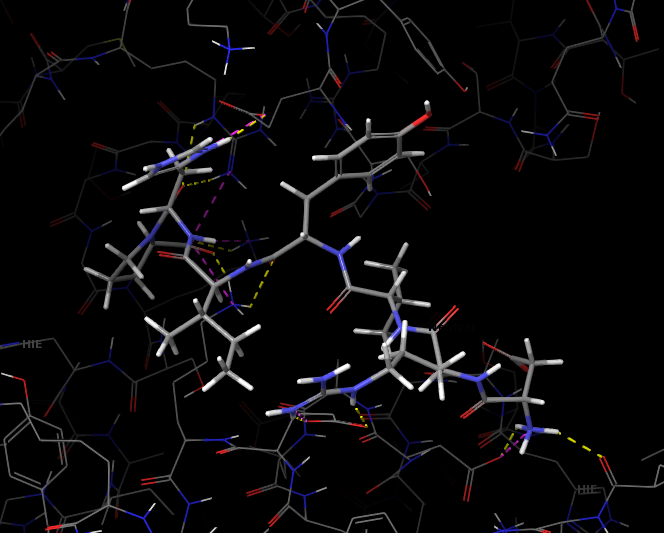
\includegraphics[scale=0.5]{docking_EOS100380.png}}
	\subcaptionbox{%
		\label{subfig:EOS100380_s}}{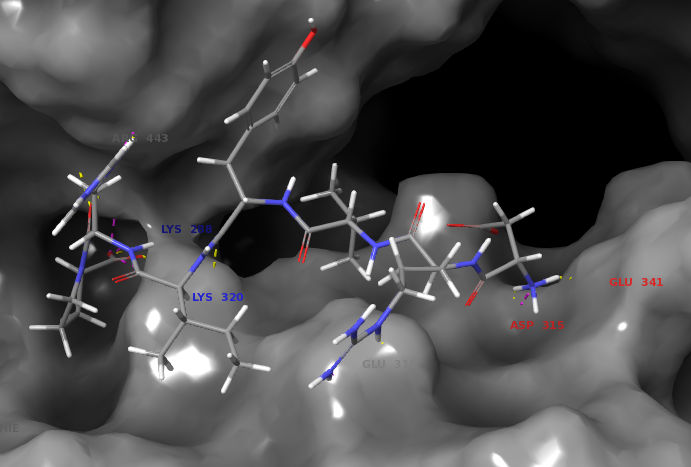
\includegraphics[scale=0.57]{docking_EOS100380_surface.png}}
	\caption{Molecular docking of the top scoring ligand with Glide. The result of the docking process with the top scoring ligand (ECBD ID: EOS100380) is shown with focus on \subref{subfig:EOS100380}) the specific interactions between ligand and receptor protein and \subref{subfig:EOS100380_s}) position within the binding pocket. The different interactions between the two molecules are coloured depending on type. Hydrogen bonds are shown as yellow and salt bridges as violet.}\label{fig:docking_EOS100380}
\end{figure}

% for appendix
\begin{figure}[htp]
	\centering
	\captionsetup[subfigure]{skip=-20pt,position=top,labelfont=bf,labelformat=parens,singlelinecheck=false}
	\subcaptionbox{%
		\label{subfig:ADP}}{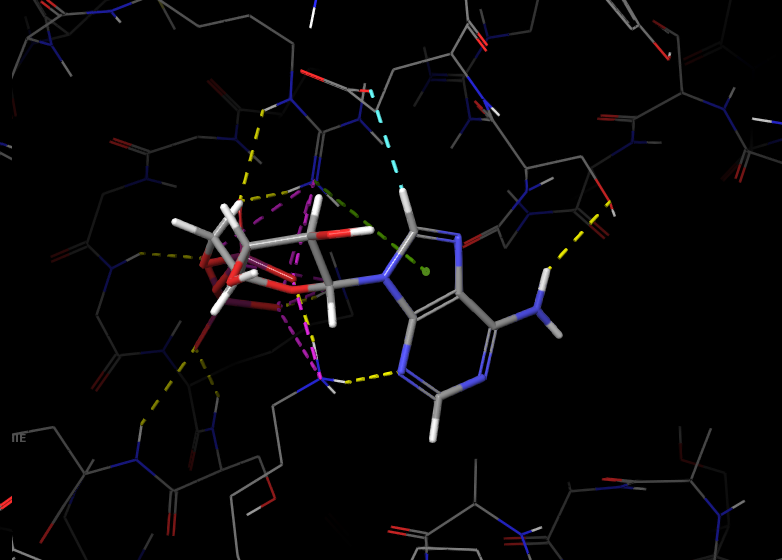
\includegraphics[scale=0.45]{docking_adp.png}}
	\subcaptionbox{%
		\label{subfig:ADP_s}}{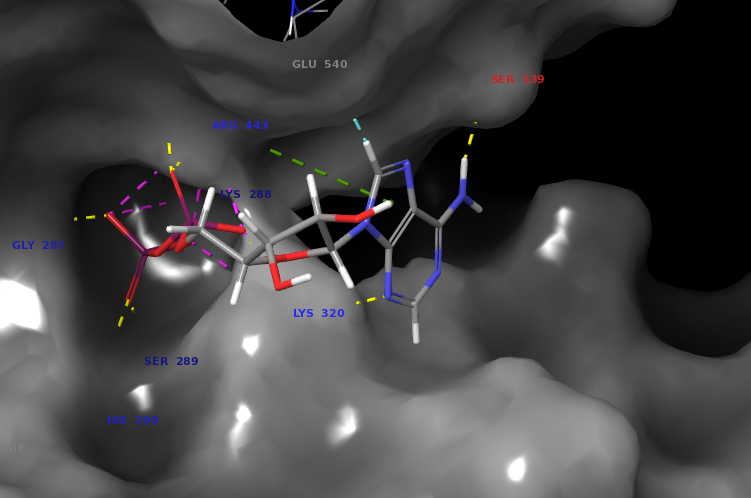
\includegraphics[scale=0.5]{docking_ADP_surface.png}}
	\caption{Molecular docking of the ADP with Glide. The result of the docking process with ADP is shown with focus on \subref{subfig:ADP}) the specific interactions between ligand and receptor protein and \subref{subfig:ADP_s}) position within the binding pocket. The different interactions between the two molecules are coloured depending on type. Hydrogen bonds are shown as yellow, salt bridges as violet, aromatic hydrogen bonds as blue and pi-cation as green.}\label{fig:docking_ADP}
\end{figure}


\subsection{Comparison of AutoDock Vina results}
%This part only makes sense if they actually used the same pocket? Don't think they used the same 6zsl structure ...
The Team Sorbonne5 also used AutoDock Vina for the docking of ligands from the pilot library of the ECBD database. Most of these ligands were also included in the former mentioned analysis. With the exception of two it is possible to map the top 10 ligands from Sorbonne to results of the analysis. Only one of their top scorers is included in the 100 preselected ligands. Their first ranked ligand with the affinity score -11.1 has a corresponding rank of 63. The remaining 7 were mapped to lower ranks starting with 123 and ending with up to 2626.

\FloatBarrier

\section{Discussion and Outlook}

\section{Supplementary Material}

\pagebreak
\FloatBarrier
\renewcommand{\bibname}{References}  % damit Literatuverzeicnis mit "References" betitelt
\printbibliography
\end{document}
